% roofline_r3.tex: generado por tools/report_c1.py desde docs/mediciones/p7/cotas/roofline.tex y c1/ops_roofline.txt.
% Ejes en log10: x de 0,01 a 100 Op/B, y de 0,1 a 100 MOPS.
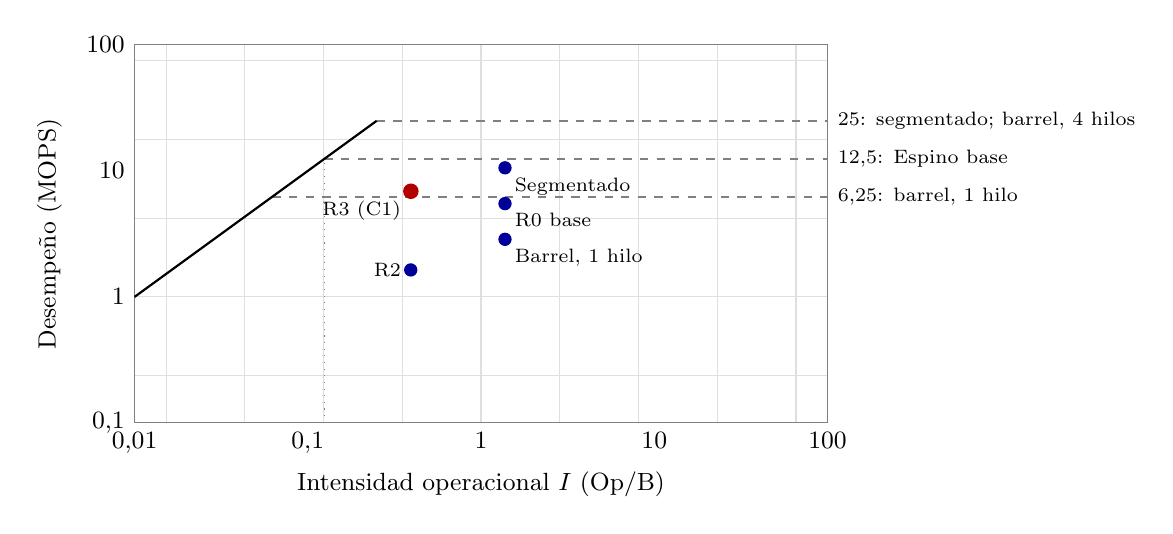
\begin{tikzpicture}[x=2.2cm,y=1.6cm,font=\small]
  \draw[gray!25] (-2,-1) grid (2,2);
  \draw[gray] (-2,-1) rectangle (2,2);
  \node[below] at (-2,-1) {$0{,}01$};
  \node[below] at (-1,-1) {$0{,}1$};
  \node[below] at (0,-1) {$1$};
  \node[below] at (1,-1) {$10$};
  \node[below] at (2,-1) {$100$};
  \node[left] at (-2,-1) {$0{,}1$};
  \node[left] at (-2,0) {$1$};
  \node[left] at (-2,1) {$10$};
  \node[left] at (-2,2) {$100$};
  \node[below=5mm] at (0.0,-1) {Intensidad operacional $I$ (Op/B)};
  \node[rotate=90,above=8mm] at (-2,0.5) {Desempeño (MOPS)};
  \draw[gray,dashed,thick] (-1.2041,0.7959) -- (2,0.7959) node[right,black,font=\scriptsize] {6{,}25: barrel{,} 1 hilo};
  \draw[gray,dashed,thick] (-0.9031,1.0969) -- (2,1.0969) node[right,black,font=\scriptsize] {12{,}5: Espino base};
  \draw[gray,dashed,thick] (-0.6021,1.3979) -- (2,1.3979) node[right,black,font=\scriptsize] {25: segmentado; barrel{,} 4 hilos};
  \draw[black,thick] (-2,0.0000) -- (-0.6021,1.3979);
  \draw[gray,dotted] (-0.9031,-1) -- (-0.9031,1.0969);
  \filldraw[blue!60!black] (0.1383,0.7404) circle (2.2pt) node[below right,font=\scriptsize,black] {R0 base};
  \filldraw[blue!60!black] (0.1383,1.0244) circle (2.2pt) node[below right,font=\scriptsize,black] {Segmentado};
  \filldraw[blue!60!black] (0.1383,0.4571) circle (2.2pt) node[below right,font=\scriptsize,black] {Barrel, 1 hilo};
  \filldraw[blue!60!black] (-0.4058,0.2140) circle (2.2pt) node[left,font=\scriptsize,black] {R2};
  \filldraw[red!70!black] (-0.4049,0.8385) circle (2.6pt) node[below left,font=\scriptsize,black] {R3 (C1)};
\end{tikzpicture}
